\subsection{Feed-forward networks}  \label{hmc_forward}

Feed-forward neural networks are formed by nodes that are connected as a directed acyclic graph (DAG), meaning that there are no cycles. Multi-layer perceptrons, the first kind of neural networks to arise, are a kind of feed-forward networks, where the layers have threshold activation.

\subsubsection{HMC Networks}

\cite{wehrmann2018hierarchical} presents a feed-forward architecture that outperforms previous \acrshort{hmc} approaches for a variety of use cases and datasets. The network comprises one layer per level in the subject hierarchy, each outputting its own local loss. These losses are then added to the global loss, after being weighted. How important local losses are is case-dependent. Therefore, the weight parameter can be adjusted.

Each layer also receives the original input, as shown in figure \ref{fig:hmcn-f}. This allows each layer to associate features from the input to the classes of the hierarchy level it represents. Thus, a layer learns features for a specific level of the subject hierarchy by processing both the original input and the output of the previous layer, i.e. the previous level of the hierarchy. According to the authors, introducing local losses feeds the network with specific local information that would otherwise be ignored, and prevents dead neurons (i.e. neurons with weight and bias close to zero) because of the increased gradient signal, which also accelerates convergence.

As is common in the multi-label setting, the authors have also picked binary cross-entropy as the loss function. Training is controlled by the Adam optimizer and a learning rate of $10^{-3}$. They used ReLU activation functions for all hidden neurons and sigmoid for the output neurons. Batches are normalized and their parameters are dropped out with a probability of 60 \% to avoid overfitting.

\begin{figure}
    \centering
    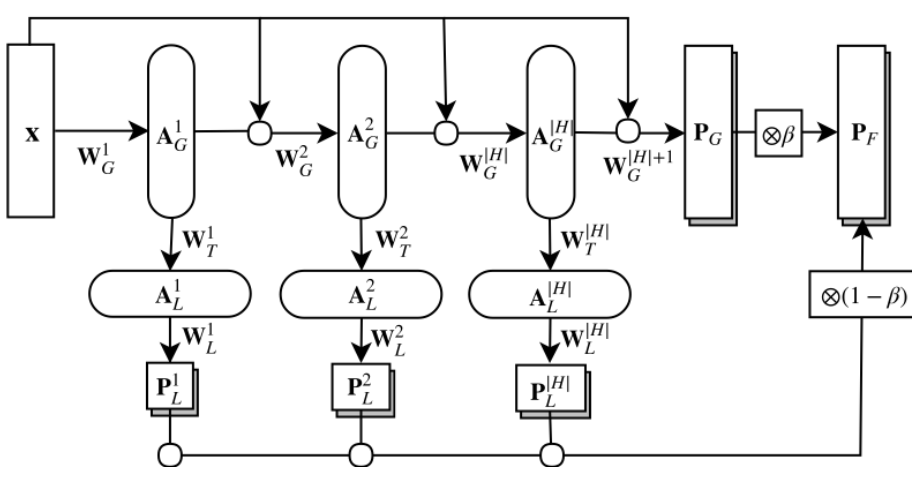
\includegraphics[width=.8\textwidth]{figures/hmc/hmcn-f.png}
    \caption{Architecture of the feed-forward HMC network from \cite{wehrmann2018hierarchical}.}
    \label{fig:hmcn-f}
\end{figure}

\subsubsection{Coherent HMC Networks}

Another feed-forward architecture was proposed in \cite{giunchiglia2020coherent}, which outperformed the architecture presented above in 17 out of 20 datasets, with a much simpler architecture. Instead of introducing local losses for the levels of the hierarchy, this approach enforces the hierarchy on the assignment probabilities by modifying the probabilities of subjects if one of their descendants has higher probability.

For example, if a document is assigned the subject \textit{k-nearest neighbors} with probability $0.7$, the probability of \textit{clustering algorithms} should at least be $0.7$. The authors ensure this is the case by picking for each class the maximum probability between its own probability and the probabilities of its descendants in the hierarchy. Formally, they introduce this constraint in the architecture with an additional layer called \acrfull{mcm}, which, for each subject, picks the maximum probability between its own and that of its descendants. Given a subject $A$ and its descendant $B$, for which a model outputs probabilities $p_A$ and $p_B$, the \acrshort{mcm} outputs the following probabilities for each node:

\begin{align*} 
    & MCM_B = p_B \\ 
    & MCM_A = \max(p_A, MCM_B)
\end{align*}

Their second contribution is a modification of the \acrfull{bce} loss function, which doesn't take into account the dependencies between labels. Their loss function incentivizes the model to respect the subject hierarchy, i.e. that subjects should not be assigned probabilities lower than the probabilities of its descendants. This loss function, called \acrfull{mcl}, can be defined for the two nodes $A$ and $B$ described above as follows:

\begin{align*} 
    & MCL_B = -y_B \ln(MCM_B) - (1 - y_B) \ln(1 - MCM_B) \\ 
    & MCL_A = -y_A \ln(\max(p_A, p_B \cdot y_B)) - (1 - y_A) \ln(1 - MCM_A)
\end{align*}

The loss for the descendant subject $B$ is computed exactly as in the \acrshort{bce} loss function, using $MCM_B$ instead of the model's output $p_B$. Note that $y_A, y_B \in {0, 1}$ are the true labels of the subjects $A$ and $B$ for a given document. The loss for the ancestor subject $A$ differs from the \acrshort{bce} loss in that in the first logarithmic term. In fact, it only changes when the subject $B$ should be assigned to the document (i.e. $y_b = 1$). Then, the loss of its ancestor $A$ takes the max function takes the maximum between $p_A$ and $p_B$ for the first logarithmic term of its loss.

For example, if the descendant subject $B$ had a higher probability than its ancestor $A$ in the model output ($p_B > p_A$) and only $A$ should be assigned to the document ($y_A = 1, y_B = 0$), the \acrshort{bce} loss would wrongly output that $p_B$ should be increased and $p_A$ kept as is. MCL, on the other hand, outputs the right losses, stating that $p_A$ should be increased and $p_B$ decreased, so the hierarchy is not violated.